\subsection{Aufgabenstellung und Versuch}

Für das Subsystem Steuerung mit H-Brücke wurden folgenden Ein- und Ausgänge
definiert.\\

\begin{itemize}
    \item ($In_1$) Die Eingangs oder Betriebsspannung $U_H$
    \item ($In_2$) Der Momentanstrom $I_{ist}$
    \item ($In_3$) Der angestrebte Strom $I_{soll}$
    \item ($Out_1$) Die Spannung die über dem Motor abfällt $U_{Motor}$
\end{itemize}


\begin{figure}[H]
    \centering
    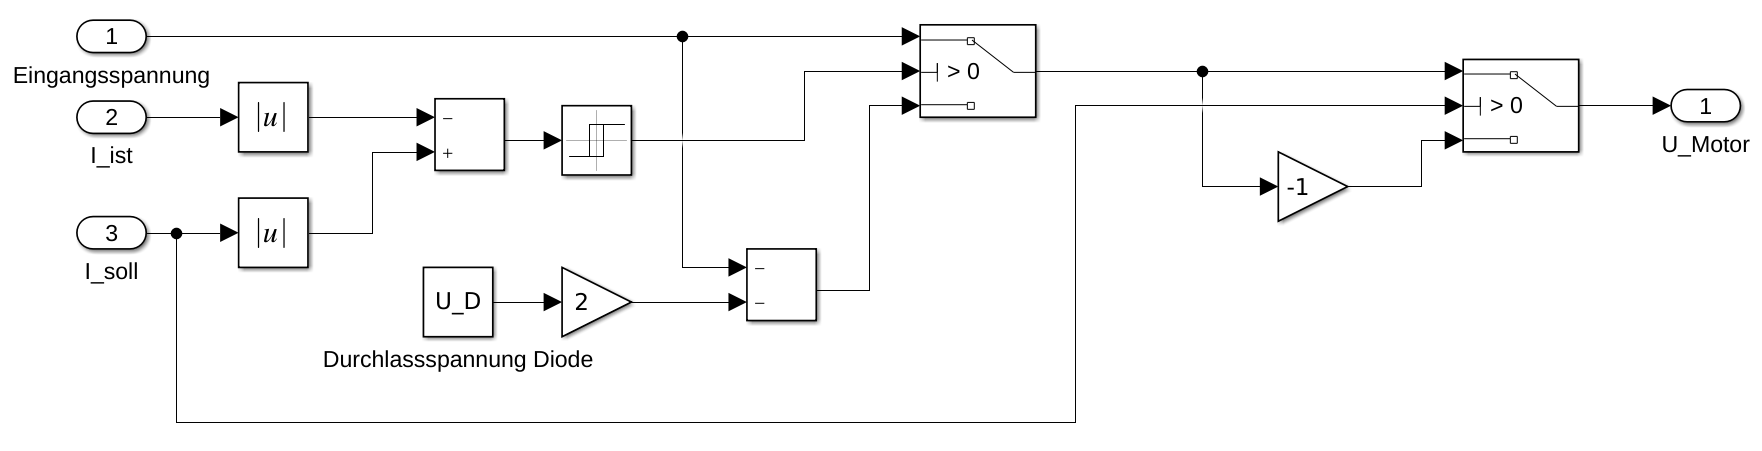
\includegraphics[width=1\textwidth]{hbridge_modell.png}
    \caption{Subsystem Steuerung mit H-Brücke}
    \label{fig:Subsystem H-Bridge}
\end{figure}